% Mid-submission report -- Team Ugh (ACL format, final mode)
% Overleaf: upload acl_latex.tex, custom.bib, acl.sty, acl_natbib.bst and
% figures/fig_primary_comparisons.pdf (keep it inside a folder named figures);
% compile with pdfLaTeX. All numbers come from ANLP_Ugh/outputs/analysis/.
\documentclass[11pt]{article}

\usepackage[final]{acl}

\usepackage{times}
\usepackage{latexsym}
\usepackage[T1]{fontenc}
\usepackage[utf8]{inputenc}
\usepackage{microtype}
\usepackage{inconsolata}
\usepackage{graphicx}
\usepackage{booktabs}
\usepackage{multirow}
\usepackage{amsmath}
\usepackage{amssymb}
\usepackage{xcolor}
\usepackage{tikz}
\usetikzlibrary{positioning,arrows.meta,calc}

\definecolor{cM1}{HTML}{2A78D6}
\definecolor{cM2}{HTML}{EB6834}
\definecolor{cM3}{HTML}{EDA100}
\definecolor{cM4}{HTML}{E87BA4}

\newcommand{\DET}{\textsc{det}}
\newcommand{\TYPE}{\textsc{type}}
\newcommand{\LVR}{\mathrm{LVR}}

\title{Structure over Scale: Hierarchy-Constrained Modeling for\\English Online Polarization Detection\\[0.3em]
\large Mid-Submission Report}

\author{Team \textit{Ugh} \\
  International Institute of Information Technology, Hyderabad \\
  \texttt{\{durga.nebhrajani, rakshitaggarwal.a, manav.beriwal\}@students.iiit.ac.in}}

\begin{document}
\maketitle

% ===================================================================
\begin{abstract}
In SemEval-2026 Task~9, a text is polarized exactly when at least one
polarization type applies to it. Most shared-task systems still predict
detection and type separately and repair contradictions afterwards. We study
whether this hierarchy should be built into the model. On the English data,
four conditions share one DeBERTa-v3-base encoder: independent models (M1),
a multi-task model (M2), post-hoc gating of M2 (M3), and M4-core, which
derives detection from the type probabilities with a differentiable noisy-OR.
We ran 100 training runs (5 folds $\times$ 5 seeds) and compared models with
paired bootstrap tests. Unconstrained models contradict the hierarchy on 62\%
of texts; M3 and M4-core never do. M4-core does not improve the pre-declared
metrics over M1 or M2 (RQ1), and it ties with post-hoc gating at equal
consistency (RQ2). The analysis explains why. M4-core detects more polarized
texts but its threshold calibration ignores neutral texts, so it raises false
alarms. It also concentrates evidence in the dominant Political label and
weakens rare labels. Gating, in turn, deletes 23\% of correct type labels.
These findings shape the plan for the final submission.
\end{abstract}

% ===================================================================
\section{Introduction}

Online polarization is language that divides people into opposing groups
through hostility, stereotyping, or exclusion. Detecting it is hard because
the signal is contextual: political words alone do not make a text
polarized, and one text can attack several groups at once.
SemEval-2026 Task~9 (POLAR) splits the problem into two related decisions
\citep{naseem-etal-2026-semeval}. \textbf{\DET{}} (Subtask~1) asks whether a
text is polarized. \textbf{\TYPE{}} (Subtask~2) asks which of five
dimensions it targets: Political, Racial/ethnic, Religious, Gender/sexual
identity, or Other.

The two decisions are \emph{nested}. Type labels exist only for polarized
texts, so a text is polarized if and only if at least one type applies.
Standard multi-task models ignore this. They put separate heads on a shared
encoder, and nothing stops them from predicting ``not polarized'' together
with a type, or ``polarized'' with no type. Shared-task teams noticed these
contradictions \citep{guo-chang-2026-yeze} and fixed them with rules applied
after prediction \citep{lin-etal-2026-nycu,maharjan-etal-2026-sagarmatha}.
\citet{maharjan-etal-2026-sagarmatha} note that their hierarchical
constraint ``slightly limits raw multi-label recall''.

Our project asks whether the hierarchy should instead be part of the model.
Our structured model, M4-core, has no separate detection head: the
probability that a text is polarized is computed from the five type
probabilities, so contradictions cannot occur. This report covers the first
stage of the project, which answers two questions:
\begin{itemize}\setlength\itemsep{1pt}
\item \textbf{RQ1.} Does deriving \DET{} from \TYPE{} improve \DET{} and
\TYPE{} macro-F1 over independent models and multi-task learning?
\item \textbf{RQ2.} At equal consistency, does building the hierarchy into
training keep more \TYPE{} recall than fixing outputs afterwards?
\end{itemize}

\paragraph{Progress summary.}
We built a complete, tested pipeline and ran a controlled comparison: 100
training runs plus 75 derived conditions, with paired statistics. The
answers are clear but not the ones we expected. RQ1 is \emph{not
supported}: M4-core is below both baselines on the pre-declared metrics.
RQ2 is \emph{inconclusive}: M4-core and post-hoc gating tie. Our analysis
traces both outcomes to specific, fixable causes and to a limit that any
consistent model must face. These findings shape the remaining work: a decoder extension, a new
parent-to-child model (RQ5), and the two research questions kept from our
proposal (\S\ref{sec:future}). Our code is at
\url{https://github.com/Rakshitagg06/ANLP_Ugh}, and all training runs are
logged on Weights \& Biases (\S\ref{sec:setup}).

% ===================================================================
\section{Problem Statement}
\label{sec:problem}

\paragraph{Task.}
Each input is an English text $x$. The gold labels are a detection label
$d \in \{0,1\}$ and a type vector $\mathbf{t} \in \{0,1\}^5$. The gold data
satisfy the hierarchy exactly:
\begin{equation}
d = 1 \iff \textstyle\bigvee_{k=1}^{5} t_k = 1 .
\label{eq:hier}
\end{equation}
A system outputs hard predictions $\hat d$ and $\hat{\mathbf t}$.

\paragraph{Consistency.}
A prediction is \emph{consistent} if it satisfies Eq.~\ref{eq:hier}. We
measure violations with a symmetric version of the Logical Violation Rate
(LVR). \citet{maharjan-etal-2026-sagarmatha} defined LVR for manifestations
(Subtask~3) predicted on texts classified as non-polarized; we adapt it to
the \DET{}/\TYPE{} pair and count both directions:
\begin{equation}
\LVR = \frac{1}{N}\sum_{i=1}^{N}\mathbf{1}\big[\hat d_i \neq
\textstyle\bigvee_k \hat t_{ik}\big],
\end{equation}
split into \textbf{LVR-A} ($\hat d=0$ but some $\hat t_k=1$) and
\textbf{LVR-B} ($\hat d=1$ but every $\hat t_k=0$).

\paragraph{Goal and research questions.}
We want models that are accurate \emph{and} consistent. Before running any
experiment, we fixed two hypotheses:
\begin{itemize}\setlength\itemsep{1pt}
\item \textbf{H1 (RQ1).} The structured model M4-core has higher \DET{}
macro-F1 and higher \TYPE{} macro-F1 than both M1 and M2.
\item \textbf{H2 (RQ2).} At equal consistency (LVR $=0$), M4-core has
higher \TYPE{} macro-F1 and macro-recall than post-hoc gating (M3).
\end{itemize}
These six comparisons form one pre-declared test family.

\paragraph{Scope.}
This stage covers English Subtasks~1--2 and uses cross-validation on the
official training set. Label-aware representations and the comparison with
very large models, both planned in our proposal, move to the final stage.

% ===================================================================
\section{Literature Review}
\label{sec:lit}

\paragraph{The POLAR benchmark.}
SemEval-2026 Task~9 covers 22 languages and received submissions from 67
teams, with 69 system papers \citep{naseem-etal-2026-semeval}. The English
data have 3{,}222 training, 160 development and 1{,}452 test texts. Two facts
from the task paper shaped our design. First, English annotator agreement
is only moderate (Fleiss' $\kappa = 0.39$), so some labels are genuinely
debatable. Second, the headroom differs between subtasks. The best English
\DET{} score is 0.825 against a baseline of 0.773, while the best \TYPE{}
score is 0.532 against 0.347. Detection is close to saturated; type
classification is where improvement is most needed.

\paragraph{How teams solved the task.}
Large generative models dominated: the Qwen family was used by 31\% of
systems, LLaMA by 20\%, Gemma/Gemini by 19\%, and BERT-style encoders by
only 7\% \citep{naseem-etal-2026-semeval}. The best English systems
fine-tuned 12B--27B models
\citep{tangkulung-tsuruoka-2026-utokyo,lin-etal-2026-nycu}.
\citet{tangkulung-tsuruoka-2026-utokyo} predict all labels in a single
forward pass, which they report reduces error propagation compared with
multi-step decoding. Encoder systems remain competitive.
\citet{daniyal-etal-2026-msqrd} fine-tune BERT-based models, and
\citet{tran-2026-uit} use DeBERTa as a high-recall filter before an LLM
assigns fine-grained labels. \citet{bokaei-etal-2026-smash} combine encoder
ensembles with thresholds tuned on out-of-fold predictions.
\citet{orsanigo-etal-2026-digis} use multi-task learning across the
subtasks, and \citet{nestor-etal-2026-polarizedteam} add label-wise
attention. This literature shows that a 184M-parameter encoder is a
reasonable base for a controlled study, even if it is not the strongest
system.

\paragraph{The hierarchy in POLAR systems.}
Several teams met the hierarchy, each with a different fix.
\citet{guo-chang-2026-yeze} train the subtasks separately, observe that
independent modelling ``causes hierarchical violations'', and suggest
post-hoc gating or hierarchical calibration as future work.
\citet{lin-etal-2026-nycu} repair one direction with a rule: if a text is
predicted polarized but no type is predicted, they assign the Other label.
\citet{mohammad-2026-polafusion} use a binary gatekeeper in front of
specialist classifiers trained only on polarized content.
\citet{djamai-etal-2026-namaa} use their Subtask~1 encoder as a hard filter
before type classification for Arabic. \citet{iannielli-etal-2026-minds}
introduce a two-stage cascade to reduce false positives under class
imbalance. The most explicit treatment is by
\citet{maharjan-etal-2026-sagarmatha}. They feed detached (stop-gradient)
Subtask~1 and~2 predictions to the manifestation head, enforce
$\hat y_{S1}=0 \Rightarrow \hat y_{S2}=0, \hat y_{S3}=0$ at inference, and
report violation rates as high as 33\% for their ensemble. On English, their
hierarchical variant scores 0.826 on \DET{} and 0.506 on \TYPE{}, against
0.752 and 0.511 for their non-hierarchical variant. In every one of these
systems the hierarchy acts \emph{after} prediction, or between separately
trained stages.

\paragraph{Multi-task learning.}
Sharing an encoder between related tasks can help both
\citep{caruana1997}, and the loss weights can be learned
\citep{kendall2018}. Sharing can also hurt: \citet{guo-chang-2026-yeze}
report negative transfer when sparse fine-grained labels share a model with
detection. \citet{le-phung-2026-alphalyrae} found that initialising the
type model from detection weights barely changed the result on Chinese
(0.8312 with it, 0.8316 without). Sharing parameters alone does not appear to transfer the
hierarchy.

\paragraph{Hierarchies and logical constraints.}
Outside POLAR, hierarchical classification is well studied.
\citet{silla2011survey} survey the field and describe how top-down systems
propagate an error at a parent node to all its children, which is exactly
the risk of post-hoc gating. \citet{giunchiglia2020} build hierarchy
consistency into the network and its loss rather than repairing outputs.
\citet{xu2018semantic} derive a training loss from logical constraints, and
\citet{giunchiglia2022survey} survey where constraints can be placed: in the
architecture, in the loss, or at inference. Our M4-core uses a noisy-OR, a
classic model of several independent causes producing one effect
\citep{pearl1988}. Label-wise attention for multi-label text classification
goes back to \citet{mullenbach-etal-2018-explainable}.

\paragraph{Thresholds and evaluation.}
Most POLAR systems tuned per-label thresholds
\citep{naseem-etal-2026-semeval}, and the F1-optimal threshold of a
classifier depends on its calibration \citep{lipton2014thresholding}. We
therefore treat threshold tuning as part of each model. All models use the
same \TYPE{} threshold grid; M1 and M2 also tune a \DET{} threshold, while
M4-core has none. For statistics we follow the paired bootstrap of
\citet{koehn-2004-statistical}, correct for multiple tests with
\citet{holm1979}, and build folds with multi-label stratification
\citep{sechidis2011}.

\paragraph{Gap and viability.}
No POLAR system makes the detection decision a \emph{function} of the type
predictions, and none compares post-hoc and training-time consistency under
one controlled setup. That is the gap we address. The study is viable: the
gold data satisfy the hierarchy exactly, the encoder is small enough to run
100 training runs in 3.9 GPU-hours (\S\ref{sec:setup}), and the shared-task
literature supplies the baselines and metrics we need.

% ===================================================================
\section{Models}
\label{sec:models}

\begin{figure}[t]
\centering
\resizebox{\columnwidth}{!}{%
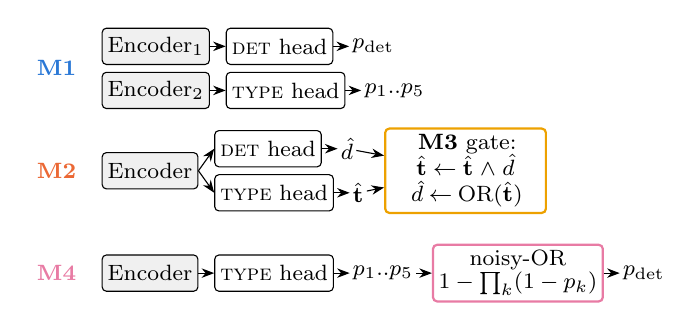
\begin{tikzpicture}[
  font=\footnotesize, node distance=2.4mm and 2mm,
  box/.style={draw, rounded corners=1.5pt, minimum height=4.6mm, inner sep=2pt, align=center},
  enc/.style={box, fill=gray!12, minimum width=11mm},
  head/.style={box, minimum width=10mm},
  res/.style={inner sep=1pt},
  arr/.style={-{Stealth[length=1.6mm]}, thin},
  lbl/.style={font=\footnotesize\bfseries, anchor=east}
]
\node[lbl, text=cM1] (l1) at (0,0) {M1};
\node[enc, right=2mm of l1, yshift=2.8mm] (e1a) {Encoder$_1$};
\node[head, right=of e1a] (h1a) {\DET{} head};
\node[res, right=of h1a] (o1a) {$p_{\text{det}}$};
\node[enc, right=2mm of l1, yshift=-2.8mm] (e1b) {Encoder$_2$};
\node[head, right=of e1b] (h1b) {\TYPE{} head};
\node[res, right=of h1b] (o1b) {$p_1..p_5$};
\draw[arr] (e1a)--(h1a); \draw[arr] (h1a)--(o1a);
\draw[arr] (e1b)--(h1b); \draw[arr] (h1b)--(o1b);
\node[lbl, text=cM2] (l2) at (0,-13mm) {M2};
\node[enc, right=2mm of l2] (e2) {Encoder};
\node[head, right=of e2, yshift=2.8mm] (h2a) {\DET{} head};
\node[head, right=of e2, yshift=-2.8mm] (h2b) {\TYPE{} head};
\node[res, right=of h2a] (o2a) {$\hat d$};
\node[res, right=of h2b] (o2b) {$\hat{\mathbf t}$};
\draw[arr] (e2.east)--(h2a.west); \draw[arr] (e2.east)--(h2b.west);
\draw[arr] (h2a)--(o2a); \draw[arr] (h2b)--(o2b);
\node[box, draw=cM3, thick, right=4mm of $(o2a)!0.5!(o2b)$, text width=19mm] (g)
  {\textbf{M3} gate:\\ $\hat{\mathbf t}\!\leftarrow\!\hat{\mathbf t}\wedge\hat d$\\ $\hat d\!\leftarrow\!\mathrm{OR}(\hat{\mathbf t})$};
\draw[arr] (o2a)--(g); \draw[arr] (o2b)--(g);
\node[lbl, text=cM4] (l4) at (0,-26mm) {M4};
\node[enc, right=2mm of l4] (e4) {Encoder};
\node[head, right=of e4] (h4) {\TYPE{} head};
\node[res, right=of h4] (o4) {$p_1..p_5$};
\node[box, draw=cM4, thick, right=of o4] (n4) {noisy-OR\\[-1pt]$1-\prod_k(1-p_k)$};
\node[res, right=2mm of n4] (d4) {$p_{\text{det}}$};
\draw[arr] (e4)--(h4); \draw[arr] (h4)--(o4); \draw[arr] (o4)--(n4); \draw[arr] (n4)--(d4);
\end{tikzpicture}}
\caption{The four conditions. All use DeBERTa-v3-base with mean pooling and
linear heads. M3 is not trained: it rewrites M2's predictions. M4-core has
no \DET{} head; detection is computed from the type probabilities, so the
hierarchy always holds.}
\label{fig:models}
\end{figure}

All models use DeBERTa-v3-base \citep{he2023debertav3} (184M parameters),
mean pooling over tokens, dropout 0.1 and linear heads
(Figure~\ref{fig:models}). Let $p_k$ be the predicted probability of type
$k$. Type labels are undefined for non-polarized texts, so the \TYPE{} loss
is a weighted binary cross-entropy (BCE) computed only on gold-polarized
texts, with per-label positive weights.

\paragraph{M1 (independent).}
Two separately trained encoders, one for \DET{} and one for \TYPE{}, as in
\citet{guo-chang-2026-yeze}. Their outputs are joined without any
consistency rule. M1 has 368M parameters.

\paragraph{M2 (shared multi-task).}
One encoder with a \DET{} head and a \TYPE{} head, trained with
$\mathcal L = \mathrm{BCE}_{\text{det}} + \lambda\,\mathcal L_{\text{type}}$
and $\lambda=1$. Nothing links the two heads.

\paragraph{M3 (post-hoc gating).}
M3 is derived from M2's predictions and reuses M2's thresholds. It applies
the inference rule of \citet{maharjan-etal-2026-sagarmatha} to the type
labels: if $\hat d = 0$, all types are set to 0 (\emph{one-way}). The
\emph{symmetric} variant then sets $\hat d \leftarrow \bigvee_k \hat t_k$,
which guarantees $\LVR = 0$.

\paragraph{M4-core (noisy-OR).}
The same encoder and \TYPE{} head as M2, but no \DET{} head. Detection is
\begin{equation}
p_{\text{det}} = 1-\textstyle\prod_{k=1}^{5}(1-p_k),
\label{eq:noisyor}
\end{equation}
the probability that at least one type applies, computed in log space for
numerical stability. It is trained with the same loss as M2. On a
non-polarized text the \DET{} loss pushes \emph{every} type probability
down, which supervises the type head exactly where the \TYPE{} loss is
masked. At inference, $\hat t_k = \mathbf 1[p_k \ge \tau_k]$ and
$\hat d = \bigvee_k \hat t_k$, so $\LVR = 0$ by construction. The word
``core'' marks that it keeps M2's head design, so M3 and M4-core differ only
in where the hierarchy is enforced.

% ===================================================================
\section{Experimental Setup}
\label{sec:setup}

\paragraph{Data.}
All results use out-of-fold predictions on the 3{,}222 English training
texts: 1{,}175 polarized and 2{,}047 not. Type support is Political 1{,}150,
Racial/ethnic 281, Religious 112, Gender/sexual 72 and Other 126. Among the
polarized texts, 426 have two or more types. Political appears in 98\% of
polarized texts, so it behaves almost like a copy of \DET{}. The gold labels
satisfy Eq.~\ref{eq:hier} with no exceptions. The supplied test file also
contains labels. We used them only to check the hierarchy (533 polarized,
919 not, no violations); because their provenance relative to the official
release is unconfirmed, no model is trained or scored on them. One training
text also appears in the test file under a different id; it does not affect
our cross-validation. The 160-text development set is too small to compare
rare labels and was not used.

\paragraph{Protocol.}
We use one fixed five-fold split, stratified over all six labels
\citep{sechidis2011}, and five seeds (13, 21, 42, 87, 100), giving
4 trained conditions $\times$ 5 folds $\times$ 5 seeds $=$ 100 training
runs. In each run, 10\% of the training folds form an inner validation set.
Early stopping, the best epoch and all thresholds are chosen there; the
held-out fold is predicted once. Training uses AdamW
\citep{loshchilov2019} with learning rate $2\times10^{-5}$, weight decay
0.01, 10\% warm-up, effective batch size 16 and FP16, for at most 8 epochs
with patience 2. Texts are truncated to 256 tokens.

\paragraph{Thresholds.}
Each type threshold $\tau_k$ is chosen from $\{0.20, 0.25, \dots, 0.80\}$
to maximize that label's F1 on the inner-validation polarized texts. M1 and
M2 also choose a \DET{} threshold for \DET{} macro-F1. M4-core has no
\DET{} threshold.

\paragraph{Metrics.}
\DET{} macro-F1 averages the F1 of both classes. \TYPE{} macro-F1,
precision and recall average over the five labels and, as fixed before the
experiments, are computed on \emph{gold-polarized texts} only. We also
report \TYPE{} on \emph{all} texts, where a type predicted for a
non-polarized text counts as a false positive.

\paragraph{Statistics.}
For each seed, the five held-out folds form one prediction set over all
3{,}222 texts. We report the mean $\pm$ standard deviation over the five
seeds. For comparisons we use a paired bootstrap over texts (2{,}000
resamples, \citealp{koehn-2004-statistical}): each resample applies the
same texts to both models and all seeds. The six pre-declared tests are
Holm-corrected \citep{holm1979}. All other comparisons are exploratory.

\paragraph{Compute.}
All runs used one NVIDIA RTX 4060 laptop GPU. A run takes 2--3 minutes, and
the full sweep took 3.9 GPU-hours.

\paragraph{Code and experiment logs.}
The code, configurations, saved analysis outputs and this report are
available at:
\begin{itemize}\setlength\itemsep{1pt}
\item \textbf{Code (GitHub):}\\ \url{https://github.com/Rakshitagg06/ANLP_Ugh}
\item \textbf{Weights \& Biases:}\\ \url{https://wandb.ai/rakshitagg06-iiit-hyderabad/anlp-project}
\end{itemize}
The W\&B project contains all 100 training runs, with their loss curves,
configurations, and saved predictions and metrics.

% ===================================================================
\section{Results}
\label{sec:results}

\begin{table*}[t]
\centering\small
\begin{tabular}{@{}lrccccccc@{}}
\toprule
& & \textbf{DET} & \multicolumn{3}{c}{\textbf{TYPE}, gold-polarized texts} & \textbf{TYPE}, all texts & \multicolumn{2}{c}{\textbf{LVR} (\%)} \\
\cmidrule(lr){3-3}\cmidrule(lr){4-6}\cmidrule(lr){7-7}\cmidrule(l){8-9}
Model & Params & macro-F1 & macro-F1 & macro-P & macro-R & macro-F1 & A & B \\
\midrule
M1 (independent)   & 368M & \textbf{0.799}\,{\scriptsize$\pm$.007} & \textbf{0.543}\,{\scriptsize$\pm$.013} & \textbf{0.509}\,{\scriptsize$\pm$.024} & \textbf{0.600}\,{\scriptsize$\pm$.023} & 0.299\,{\scriptsize$\pm$.013} & 61.9 & 0.0 \\
M2 (shared MTL)    & 184M & 0.793\,{\scriptsize$\pm$.003} & 0.497\,{\scriptsize$\pm$.015} & 0.444\,{\scriptsize$\pm$.018} & 0.595\,{\scriptsize$\pm$.019} & 0.255\,{\scriptsize$\pm$.029} & 61.5 & 0.0 \\
M3 (gating)        & 184M & 0.793\,{\scriptsize$\pm$.003} & 0.453\,{\scriptsize$\pm$.022} & 0.469\,{\scriptsize$\pm$.033} & 0.468\,{\scriptsize$\pm$.036} & 0.382\,{\scriptsize$\pm$.017} & 0.0 & 0.0 \\
M4-core (noisy-OR) & 184M & 0.784\,{\scriptsize$\pm$.004} & 0.461\,{\scriptsize$\pm$.007} & 0.465\,{\scriptsize$\pm$.011} & 0.474\,{\scriptsize$\pm$.022} & \textbf{0.396}\,{\scriptsize$\pm$.008} & 0.0 & 0.0 \\
\bottomrule
\end{tabular}
\caption{\textbf{Main results} (out-of-fold over 3{,}222 texts; mean $\pm$ sd
over five seeds; best in bold). M3 is the symmetric variant; the one-way
variant has identical \TYPE{} predictions and differs on \DET{} for only two
texts in one seed. LVR-A: ``not polarized'' but a type is predicted. LVR-B:
``polarized'' but no type is predicted.}
\label{tab:main}
\end{table*}

Table~\ref{tab:main} gives the overall picture. M1 is the strongest model on
every pre-declared metric. The two consistent models, M3 and M4-core, have
lower \TYPE{} scores on gold-polarized texts, and the gap comes from recall
(about 0.47 vs.\ 0.60), not precision.

\subsection{Consistency}
The unconstrained models contradict the hierarchy on \textbf{62\%} of all
texts, almost entirely as LVR-A. M2 predicts at least one type for every one
of the 2{,}047 non-polarized texts, and M1 for 2{,}039 of them. The reason
is how their type heads are trained. The \TYPE{} loss never sees a
non-polarized text, positive weights push type probabilities up, and the
thresholds are tuned only on polarized texts. Nothing teaches these heads to
stay silent. M3 and M4-core have zero violations in every run.

\subsection{RQ1: Does noisy-OR beat M1 and M2?}
\label{sec:rq1}

\begin{table}[t]
\centering\small
\setlength{\tabcolsep}{2.5pt}
\resizebox{\columnwidth}{!}{%
\begin{tabular}{@{}llccc@{}}
\toprule
& Comparison & $\Delta$ & 95\% CI & $p_{\text{Holm}}$ \\
\midrule
\multirow{4}{*}{RQ1} & M4$-$M1 \DET{} F1 & $-$0.014 & [$-$0.023, $-$0.006] & $<$0.001 \\
 & M4$-$M1 \TYPE{} F1 & $-$0.082 & [$-$0.102, $-$0.064] & $<$0.001 \\
 & M4$-$M2 \DET{} F1 & $-$0.008 & [$-$0.016, $-$0.001] & 0.072 \\
 & M4$-$M2 \TYPE{} F1 & $-$0.036 & [$-$0.055, $-$0.019] & 0.004 \\
\midrule
\multirow{2}{*}{RQ2} & M4$-$M3 \TYPE{} F1 & +0.008 & [$-$0.009, +0.022] & 0.732 \\
 & M4$-$M3 \TYPE{} R & +0.006 & [$-$0.014, +0.023] & 0.732 \\
\bottomrule
\end{tabular}}
\caption{\textbf{Pre-declared tests.} $\Delta$ is the seed-averaged
difference; the CI is a 95\% paired bootstrap interval. \TYPE{} scores use
gold-polarized texts.}
\label{tab:primary}
\end{table}

\begin{figure}[t]
\centering
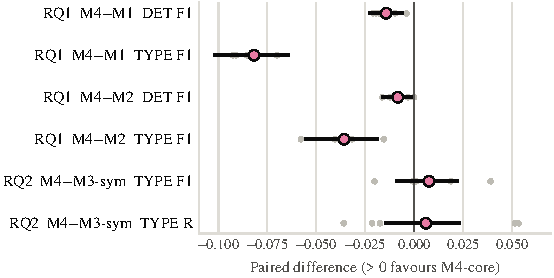
\includegraphics[width=\columnwidth]{figures/fig_primary_comparisons.pdf}
\caption{\textbf{The six pre-declared tests.} Pink: mean difference
(M4-core minus baseline). Black bar: 95\% CI. Grey: the five per-seed
differences. All RQ1 bars lie left of zero (M4-core worse); both RQ2 bars
cross zero (no detectable difference).}
\label{fig:forest}
\end{figure}

Table~\ref{tab:primary} and Figure~\ref{fig:forest} show that \textbf{H1 is
not supported}. M4-core is below M1 on both metrics and below M2 on \TYPE{};
these three differences remain significant after Holm correction, and no
seed favours M4-core. Against M2 on \DET{}, M4-core is lower in all five
seeds, but the difference is not significant after correction
($p=0.072$). Two mechanisms explain the result.

\paragraph{The \DET{} gap comes from false alarms.}
M4-core finds more polarized texts but also flags more neutral ones
(Table~\ref{tab:det}). Its \DET{} recall rises from 0.761 (M2) to 0.831,
while precision falls from 0.722 to 0.674. The cause is the decision rule.
M4-core says ``polarized'' when \emph{any} type passes its threshold, and
those thresholds were tuned only on polarized texts, so their tuning never
saw the cost of a false alarm. The Political threshold, which almost decides
detection on its own, fell to the bottom of the grid (0.20) in 19 of 25
runs. M1 and M2, by contrast, tune a dedicated \DET{} threshold for \DET{}
macro-F1. The \DET{} comparison is therefore not calibration-matched.

\begin{table}[t]
\centering\small
\setlength{\tabcolsep}{4pt}
\begin{tabular}{@{}lccccc@{}}
\toprule
Model & \DET{} P & \DET{} R & FP & FN & Neutral w/ type \\
\midrule
M1 & 0.733 & 0.761 & 325 & 280 & 2{,}039 \\
M2 & 0.722 & 0.761 & 345 & 281 & 2{,}047 \\
M3 & 0.722 & 0.761 & 345 & 281 & 345 \\
M4 & 0.674 & \textbf{0.831} & 472 & \textbf{199} & 472 \\
\bottomrule
\end{tabular}
\caption{\textbf{Detection errors} (per seed, 3{,}222 texts). P/R: precision
and recall of the polarized class. FP: neutral texts flagged as polarized.
FN: polarized texts missed. Last column: neutral texts given at least one
type.}
\label{tab:det}
\end{table}

\paragraph{The \TYPE{} gap is the price of consistency.}
Under the pre-declared metric, a type predicted for a neutral text is not
counted as an error. M1 and M2 benefit fully from this. A consistent model
cannot: on a polarized text it can only output a type if it also detects
the text, so its type recall is capped by its detection. The RQ1 \TYPE{}
test therefore compares a consistent model with inconsistent ones. When the
same predictions are scored on all texts, the ranking reverses
(Table~\ref{tab:main}): M4-core scores 0.396, against 0.299 for M1 and 0.255
for M2. The paired gains are +0.097 [+0.078, +0.114] over M1 and +0.141
[+0.121, +0.158] over M2, in all five seeds. This view is exploratory and
does not change the pre-declared verdict, but it shows that the RQ1 outcome
depends on what the metric chooses to count. We have not yet verified which
scope the official SemEval scorer uses.

\subsection{RQ2: Gating versus training-time structure}
\label{sec:rq2}

Both M3 and M4-core have zero violations, so RQ2 compares them at equal
consistency. Their pre-declared scores are statistically tied
(Table~\ref{tab:primary}). The \TYPE{} F1 difference is +0.008 with a 95\%
CI of [$-$0.009, +0.022], and the seeds split 3/5 and 2/5. \textbf{H2 is not
supported}, and neither is the opposite. The intervals do rule out large
effects: the upper end of the recall interval, +0.023, is less than a fifth
of the 0.127 recall that gating costs relative to M2.

\begin{table}[t]
\centering\small
\setlength{\tabcolsep}{3pt}
\begin{tabular}{@{}lccc@{}}
\toprule
& M3 & M4-core & M4$-$M3 [95\% CI] \\
\midrule
Coverage          & 0.768 & 0.843 & +0.075 [+0.064, +0.087] \\
Cond.\ recall     & 0.853 & 0.823 & $-$0.030 [$-$0.041, $-$0.020] \\
Micro recall      & 0.655 & 0.694 & +0.038 [+0.027, +0.049] \\
Macro recall      & 0.468 & 0.474 & +0.006 [$-$0.014, +0.023] \\
\midrule
\multicolumn{4}{@{}l}{\emph{Median $p_k$ on texts that carry label $k$ (M2 $\rightarrow$ M4-core)}} \\
\multicolumn{4}{@{}l}{Political 0.577 $\rightarrow$ 0.754 \quad Religious 0.772 $\rightarrow$ 0.419} \\
\multicolumn{4}{@{}l}{Gender 0.354 $\rightarrow$ 0.051 \quad Other 0.392 $\rightarrow$ 0.159} \\
\bottomrule
\end{tabular}
\caption{\textbf{Why RQ2 ties} (exploratory). Coverage: share of gold type
labels on texts the model detects. Conditional recall: share of those labels
it then predicts. Micro recall $=$ coverage $\times$ conditional recall. The
first three differences hold in all five seeds.}
\label{tab:decomp}
\end{table}

\paragraph{Two opposite effects cancel.}
For a consistent model, label recall equals \emph{coverage} (the share of
gold labels on texts it detects) times \emph{conditional recall} (how many
of those labels it then predicts). Table~\ref{tab:decomp} shows that the
models sit at opposite ends of this product. M3 keeps M2's discrimination
(0.853) but inherits the 23\% of labels on texts M2's detector misses.
M4-core detects more (coverage +0.075) but discriminates less well among
detected texts ($-$0.030). Both effects are consistent across all seeds. The
coverage gain falls mainly on Political, which carries two thirds of all
type labels. The discrimination loss falls on Racial/ethnic, Religious and
Other. Micro recall, which weights labels by frequency, therefore favours
M4-core (+0.038), while macro recall, which weights all labels equally,
shows a tie.

\begin{table}[t]
\centering\small
\setlength{\tabcolsep}{3pt}
\resizebox{\columnwidth}{!}{%
\begin{tabular}{@{}lrcc@{}}
\toprule
Label & $n$ & $\Delta$ recall [95\% CI] & $\Delta$ F1 [95\% CI] \\
\midrule
Political & 1{,}150 & \textbf{+0.067} [+.055, +.078] & \textbf{+0.040} [+.033, +.048] \\
Racial/ethnic & 281 & $-$0.011 [$-$.041, +.019] & \textbf{$-$0.026} [$-$.051, $-$.003] \\
Religious & 112 & $-$0.016 [$-$.059, +.026] & $-$0.006 [$-$.041, +.030] \\
Gender/sexual & 72 & \textbf{+0.064} [+.009, +.116] & +0.039 [$-$.014, +.089] \\
Other & 126 & \textbf{$-$0.073} [$-$.113, $-$.034] & $-$0.009 [$-$.039, +.019] \\
\bottomrule
\end{tabular}}
\caption{\textbf{RQ2 per label}: M4-core minus M3 on gold-polarized texts
(exploratory). Bold: the 95\% interval excludes zero.}
\label{tab:perlabel-rq2}
\end{table}

\paragraph{The tie hides per-label differences.}
Table~\ref{tab:perlabel-rq2} shows the same pattern label by label. M4-core
is clearly better on Political and recovers more of the rarest label,
Gender/sexual. It is worse on Other and less precise on Racial/ethnic. A
macro average gives each label equal weight, so these gains and losses
cancel.

\paragraph{Why M4-core weakens rare labels.}
The noisy-OR loss does two things at once (Table~\ref{tab:decomp}, bottom).
On neutral texts it pushes every type probability close to zero (median
$\le 0.012$, against up to 0.55 for M2), which is the intended effect. But
on polarized texts, the detection target can be satisfied by Political
alone, so the loss rewards raising Political and gives little reason to
raise the other heads. As a result, rare labels are suppressed even on texts
that truly have them: the median Gender probability on Gender texts falls
from 0.354 to 0.051. This is a credit-assignment problem. In
Eq.~\ref{eq:noisyor}, once one head is confident, the gradient reaching the
other heads becomes small.

\paragraph{What gating removes.}
Per seed, gating deletes 4{,}379 of the 6{,}647 type labels M2 predicts.
87.7\% of them are false alarms on neutral texts, which is gating working as
intended. But it also deletes \textbf{338 correct labels, 22.9\%} of all
correct type predictions M2 makes. Every one of them is on a polarized text
that M2's detection head missed, and on 98.7\% of those texts M2 had already
predicted at least one correct type. This is the error propagation that
\citet{silla2011survey} describe for top-down classifiers. The loss is
larger on single-label texts ($-$0.239 recall) than on multi-label texts
($-$0.161). The cost of gating therefore comes from detection misses, not
from the number of labels on a text.

% ===================================================================
\section{Progress Against the Proposal}
\label{sec:progress}

\begin{table}[t]
\centering\small
\setlength{\tabcolsep}{4pt}
\resizebox{\columnwidth}{!}{%
\begin{tabular}{@{}ll@{}}
\toprule
Proposal item & Status \\
\midrule
Stratified 5-fold CV, metrics, LVR & Done \\
M1 and M2 (5 folds $\times$ 5 seeds) & Done \\
M3 gating & Done (re-implemented) \\
M4 noisy-OR & Done as M4-core \\
Full 5$\times$5 ladder and paired tests & Done (ahead of plan) \\
Label-aware attention, Other head & Kept as RQ3 \\
TF-IDF, BERT, RoBERTa baselines & Deferred \\
Learned loss weighting & Deferred \\
Comparison with 12B--27B systems & Kept as RQ4 \\
Leaderboard claim & Not made (RQ4) \\
\bottomrule
\end{tabular}}
\caption{Status of the work planned in the proposal.}
\label{tab:progress}
\end{table}

Table~\ref{tab:progress} compares our progress with the proposal. The
controlled four-model comparison, which the proposal scheduled for
mid-October, is complete, including the full five-fold, five-seed sweep and
the significance tests. Three changes were deliberate:
\begin{itemize}\setlength\itemsep{1pt}
\item \textbf{M4 became M4-core.} The proposal's M4 combined label-aware
attention with noisy-OR. Testing both at once would make it impossible to
tell which one causes a difference, so we first isolated the hierarchy
mechanism. Label-aware attention remains RQ3.
\item \textbf{M3 was re-implemented.} Instead of adapting the released
Sagarmatha system, we applied its inference rule to our own M2, so that M3
and M4-core share the same encoder, data and thresholds.
\item \textbf{Classical baselines were deferred.} The TF-IDF, BERT and
RoBERTa baselines do not affect RQ1 or RQ2, so they come after the
controlled comparison.
\end{itemize}
We also built the infrastructure: configuration-driven training, saved
predictions, experiment tracking, an analysis pipeline that regenerates every
table, and unit tests, which caught two bugs before the main sweep.

% ===================================================================
\section{Discussion}
\label{sec:discussion}

We expected the structured model to avoid gating's recall loss because it
``discards nothing''. This was too simple: a consistent model cannot recover a
type on a text it fails to detect, and where the constraint is enforced only
changes who pays for that limit. Post-hoc gating keeps the unconstrained model's type discrimination but
inherits its detector's misses. Training-time noisy-OR detects more texts,
but its loss concentrates evidence in the dominant label and its decoder
inherits thresholds that never saw neutral text.

Three lessons follow. First, the evaluation scope matters: whether \TYPE{}
is scored on polarized texts or on all texts reverses the model ranking.
Second, calibration is part of the model. M4-core's main weaknesses come
from how its probabilities are turned into decisions, not only from how it
is trained. Third, the direction of the hierarchy matters. Deriving the
parent from the children lets a confident child switch on the parent, and
lets it absorb the credit that should reach the other children. These
lessons define the next stage.

% ===================================================================
\section{Remaining Work and Research Questions}
\label{sec:future}

RQ1 and RQ2 are closed under the frozen protocol, and their answers stay as
reported. The open question is no longer whether noisy-OR wins on the frozen
macro-F1 numbers. It is whether the consistency--recall trade-off comes from
the \emph{decoder}, from \emph{aggregating} types into detection, or from the
\emph{hierarchy itself}. The remaining work tests these in that order. It
keeps the two research questions from our proposal (RQ3 and RQ4) and adds
one new question (RQ5). All primary tests and margins will be fixed before
any new run.

\paragraph{Decoder extension (not a new RQ).}
\emph{Does M4-core improve once its thresholds see neutral texts?} In the
current code, \TYPE{} thresholds use only gold-polarized inner-validation
texts, and no inner-validation probabilities or checkpoints were saved, so a
proper test needs a code change and new runs. We will rerun M4-core (25 runs) with thresholds tuned on \emph{all}
inner-validation texts over the grid $\{0.05, 0.10, \dots, 0.80\}$, and keep
checkpoint selection on gold-polarized \TYPE{} macro-F1, so that only the
threshold rule changes. Because M3 is derived from M2, we will also rerun M2
(25 runs). Both reruns save inner-validation probabilities, which lets us
place M3 and M4-core at the same detection precision, and separately at the
same detection recall, without tuning on held-out folds. Re-thresholding the
already saved held-out predictions would tune on test data, so we will report
it only as exploratory.
\emph{Why it matters:} RQ1 traced M4-core's \DET{} loss to thresholds tuned
without neutral texts, and RQ2 compared the two consistent models at
different operating points. This is the cheapest test of whether those
results are decoding artefacts. The results will be reported beside the
frozen RQ1/RQ2 tables, not instead of them.

\paragraph{RQ5 (new): Does the direction of the hierarchy matter?}
\emph{Can a calibrated parent-to-child model improve \TYPE{} while keeping
\DET{} as good as M2's?} M4-core builds detection from the types. The new
model, M5, does the reverse. It keeps an independent \DET{} head $d$ and a
conditional type head $q_k$, and predicts $p_k = d \cdot q_k$, the
factorization $P(t_k \mid x) = P(d \mid x)\,P(t_k \mid d, x)$ implied by the
hierarchy. Low detection confidence then softly lowers every type, and a
confident type can no longer switch detection on. The \DET{} head is
trained with BCE on all texts. Because $q_k$ means $P(t_k \mid d=1, x)$, its
weighted BCE is computed on gold-polarized texts only. Thresholds are tuned
on all inner-validation texts over the same grid as the decoder extension.
We will test two decoders with the same encoder, folds and seeds:
\emph{soft}, $\hat t_k = \mathbf 1[d\,q_k \ge \tau_k]$ and
$\hat d = \mathbf 1[d \ge \tau_D]$; and \emph{hard}, which also requires
$\hat d = 1$ for any $\hat t_k = 1$. Two hypotheses are fixed in advance.
\textbf{H5a:} M5 has higher \TYPE{} macro-F1 than M2 and than the
decoder-extension M4-core, on the scoring scope fixed on Oct~2--3.
\textbf{H5b} (non-inferiority): \DET{} macro-F1 is at most $\delta=0.01$
below M2. H5b is decided by the lower end of the 95\% paired bootstrap
interval for M5$-$M2, which must lie above $-0.01$; the point estimate alone
is not enough.
\emph{Why it matters:} the decoder extension can fix M4-core's thresholds,
but not the fact that one confident type switches detection on and absorbs
the credit for the others (\S\ref{sec:rq2}). RQ5 tests whether the hierarchy
helps when it follows the direction of the label definition.

\paragraph{RQ3 (proposal): Do label-aware representations help rare labels?}
\emph{Do label-specific representations improve rare-label and multi-label
\TYPE{} performance, especially for Other?} As in our proposal, each named
type gets a learned query that attends over the tokens
\citep{mullenbach-etal-2018-explainable,nestor-etal-2026-polarizedteam}, and
Other gets a separate head on the pooled representation, since it has no
single meaning. RQ3 will run on one hierarchy variant, chosen by a fixed
keep-rule: the M5 variant that passes H5b; if both pass, the one with higher
\TYPE{} macro-F1; if neither passes, the decoder-extension M4-core. This way
a new head is not confounded with a new constraint.
\emph{Why it matters:} Gender/sexual and Other are the weakest labels for
every model (F1 below 0.30) and lose most under noisy-OR, and all five types
currently share one pooled vector. Type classification is also where the
task has the most headroom (0.532 best vs.\ 0.347 baseline).

\paragraph{RQ4 (proposal): How does a 184M model compare with 12B--27B systems?}
\emph{How does our best structured encoder compare with the much larger
systems that lead the English leaderboard, relative to model size?} We will
place our out-of-fold scores beside the published English results (0.825
\DET{}, 0.532 \TYPE{}) and state clearly that the two come from different
data splits. We will not call this a leaderboard comparison. We will compare
two models: the variant chosen by the keep-rule, trained once more with its
checkpoint kept, and the frozen M4-core. The development set will be scored
once, as a sanity check, and will not be used to choose between models. The test file stays unused until its labels are
confirmed; the one text it shares with the training set will then be left
out.
\emph{Why it matters:} it measures how much of the gap to large models a
small structured encoder closes, the ``structure over scale'' question.

\paragraph{Deferred.}
The TF-IDF, BERT and RoBERTa baselines and learned loss weighting
\citep{kendall2018} are deferred in favour of the decoder extension and RQ5.

% ===================================================================
\section{Timeline}
\label{sec:timeline}

\begin{table}[t]
\centering\small
\setlength{\tabcolsep}{3pt}
\begin{tabular}{@{}p{1.45cm}p{5.55cm}@{}}
\toprule
Dates & Work \\
\midrule
Oct~2--3 & Read the official Subtask~2 scorer and record whether later \TYPE{} scores use all texts or gold-polarized texts only. \\
Oct~4--6 & Decoder extension: change threshold selection to all inner-validation texts (grid 0.05--0.80) and save inner-validation probabilities; rerun M4-core and M2 (25 runs each); matched operating-point comparison of M3 and M4-core. \\
Oct~7--16 & RQ5: parent-to-child M5, soft and hard decoders (25 runs each); test H5a and H5b; apply the keep-rule. \\
Oct~17--23 & RQ3: label-aware heads and a separate Other head on the kept variant; single- vs.\ multi-label analysis. \\
Oct~24--27 & RQ4: kept variant (retrained with checkpoint) and frozen M4-core vs.\ published 12B--27B results; development set scored once. \\
Oct~28--31 & Error analysis of Other and neutral false alarms; final report and code release. \\
\bottomrule
\end{tabular}
\caption{Plan to the final submission (October 31). RQ1 and RQ2 are closed;
every later row is a new experiment.}
\label{tab:timeline}
\end{table}

Table~\ref{tab:timeline} gives the plan. Each 25-run condition takes about
one GPU-hour on our hardware, so the training budget is not a risk. The main
risks are scientific: M5 may lose \DET{} recall through its gate and fail
H5b, in which case RQ3 falls back to the decoder-extension M4-core; and if
the test-label question stays open, RQ4 will say so and rely on the
published numbers.

% ===================================================================
\section{Conclusion}

Unconstrained models contradict the POLAR hierarchy on most texts. A
noisy-OR model removes every contradiction but does not beat independent or
multi-task models on our pre-declared metrics, and it ties with post-hoc
gating, which itself removes almost a quarter of correct labels. We traced
these outcomes to specific, testable causes, and the final stage tests them
directly.

% ===================================================================
\section*{Limitations}
The pre-declared \TYPE{} metric scores only gold-polarized texts, which
favours unconstrained models, and we have not yet confirmed the official
scorer's scope. Detection decisions are not calibration-matched across
models, and M1 has twice the parameters of the others. Bootstrap intervals
capture variation over texts; training variation is reflected only through
five seeds, and only the six pre-declared tests are corrected for multiple
comparisons. The decomposition and probability analyses were designed after
seeing the main results. All results are English cross-validation scores
from one consumer GPU, so they are not leaderboard-comparable.

\bibliography{custom}

\end{document}
